The lower level design of the system are explained in the architecture design of the system. 

\section{Audio-DSP}
\begin{figure}[ht]
    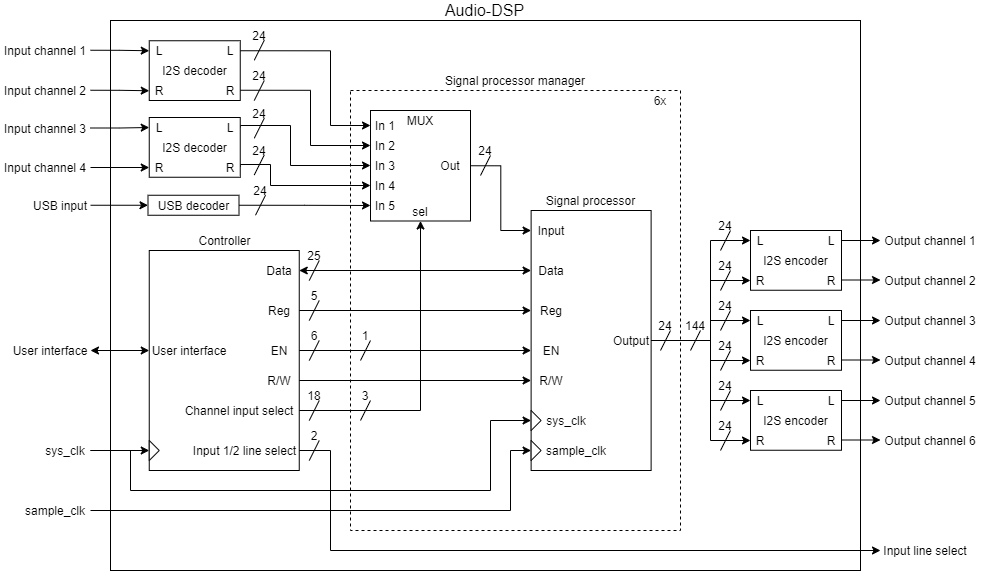
\includegraphics[width=\linewidth]{Audio-DSP architecture.png}\\    
    \caption{Top-level architecture of audio-DSP}
    \label{fig:arch-top}
\end{figure}

In figure \ref*{fig:arch-top} you see the architecture design of the Audio-DSP. Compared to the system context diagram of the Audio-DSP the block is now much more detailed. For instance the input samplers are replaced by $I^2S$ decoders and the output signals are now encoded to $I^2S$. Because most ADCs and DACs use the $I^2S$ protocol to transfer audio data it has been chosen to use the $I^2S$ protocol. The $I^2S$ encoders and decoders each have a left and right input and output. This is because the $I^2S$ protocol transfers a stereo audio signal. But this system uses mono signals. Therefore the system inputs the mono signals on the left and right inputs. This gives the system the ability to transfer two audio channels via one $I^2S$ bus.

The MUX in each of the signal processor managers is controlled via a 3-bit select line. This select line comes from the controller. For the controller to be able to handle all the multiplexers in each signal processor manager, 3-bits $\cdot$ 6 channels = 18 bits are needed. To select the RCA or 6.35mm jack input a 2-bit select line is used.

In order for the signal processor to modify the signal with various digital effects, memory is needed. This memory is stored inside the signal processor block itself. To access and modify the memory some kind of communication protocol had to be chosen in order for the controller to configure the effect parameters. For this a register based memory has been chosen.

Looking at the system requirements it is known that the user is able to adjust the position of each effect in the effects loop. Therefore the signal processor needs registers to store the position of each effect. The system must support at least five effects and should support at least twenty effects. Thus in order to fulfill all the requirements the signal processor should be able to position twenty effects. For this we would need at least 5 bits at each position. The various effects available to the user have configurable parameters. Therefore each effect also needs a register in the signal processor block. Also the equalizer settings are adjustable by the user. This means the equalizer also has a register with data.

The size of the registers can be very large. But to make the communication to the signal processor intuitive the registers will be limited to a maximum amount of bits. In order to choose the most efficient register size the registers should use most of its bits. The size of the register is of no importance for the effect and equalizer parameters as the size only affects the resolution of the parameters. But for the position register 5-bits per position are needed. Thus the register should be dividable by 5 in order to use the most of the registers bits. As there are 20 positions it is chosen to have four position registers with 5 positions (see figure \ref{fig:reg-position}).
This means the register size will be 25 bits.

% \begin{wrapfigure}[20]{r}{0.25\textwidth}
%     \centering
%     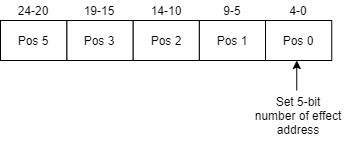
\includegraphics[width=0.25\textwidth]{Position register design}
%     \caption{Effect loop position 0 to 4 register}
%     \label{fig:reg-position}
% \end{wrapfigure}

\begin{figure}[ht]
    \centering
    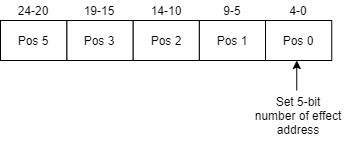
\includegraphics[width=0.4\textwidth]{Position register design}
    \caption{Effect loop position 0 to 4 register}
    \label{fig:reg-position}
\end{figure}

Now that the register size has been defined we need to define the amount of registers needed. The system has 20 effects, therefore 20 effect parameter registers. Each effect needs to be positioned in the position registers which there are four of. Then the equalizer and volume registers are left. when using 5 bits for selecting the registers we would be able to access up to 32 registers. This means that there are $32 - (20 + 4) = 8$ registers left for the equalizer and volume parameters. That is more than enough for these registers.

Thus the data bus will be 25 bits and the register selector line will be 5 bits. With these two lines every register can be accessed by the controller. Now the memory needs to know if the data needs to be read or written. This is indicated by the R/W signal. When this signal is low the memory will be written and when the signal is high the memory will be read.

It is undesired that every signal processor memory will be read or written constantly. Therefore each signal processor block has an enable. When this enable signal is high the memory can be read or written. This gives the controller the ability to read or write to only one signal processor memory at a time. And the ability to write multiple signal processor memories at once.


\subsection{Signal processor}
The signal processor has to load a new sample into the effect loop and the previous modified sample to the output on the sample frequency. The sample frequency of the Audio-DSP is 192kHz. This means that the signal processor has $\frac{1}{192 \cdot 10^3} \approx 5 \mu s$ to process the sample. With a clock of 50MHz the sample must be modified and loaded into the output within $\frac{50 \cdot 10^6}{192 \cdot 10^3}=260$ clock ticks.
% \textbf{!!!This could be different according to the new design I just made - 28/04/2023 Youri !!! }\\

When a sample has been loaded into the signal processor, it is fed into the effect processor manager (see \ref{fig:arch-signal-processor}). The effect processor manager houses multiple effects processor in series. The sample will go through these effect processors. Each effect processor can be configured to be a certain effect (see \ref{fig:arch-effect-processor}). Because the system has at least twenty effects, the amount of bits the selector needs is 5 bits.

Each effect modifies the signal by applying a transfer function to the sample. The variables in that transfer function are configured by the user via the user interface. Therefore the effect processors needs to get the variables from the controller block, which gets the variables from the register bank. After the sample has gone through all the 

\begin{figure}[ht]
    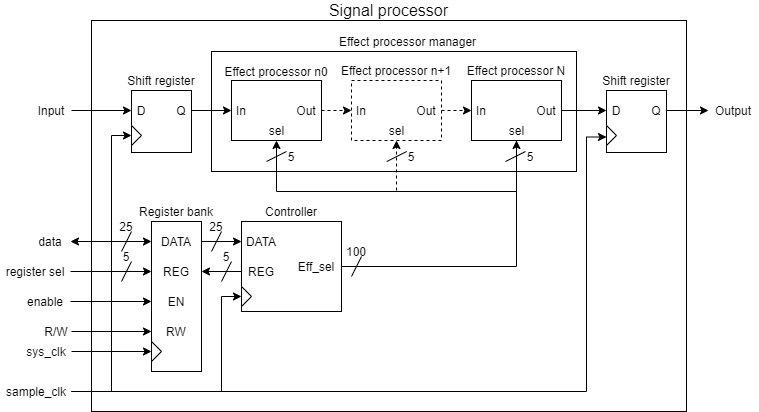
\includegraphics[width=\linewidth]{Signal processor architecture}
    \caption{Signal processor architecture}
    \label{fig:arch-signal-processor}
\end{figure}



\begin{figure}[ht]
    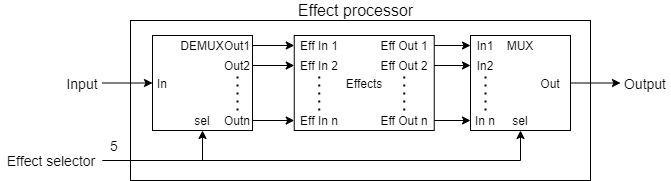
\includegraphics[width=\linewidth]{Effect processor architecture}
    \caption{Effect processor architecture}
    \label{fig:arch-effect-processor}
\end{figure}


